\documentclass[../main.tex]{subfiles}
\graphicspath{{\subfix{../images/}}}
\begin{document}

  \chapter{Metacognitive Exercises}\label{metacognitive}
  The metacognitive\footnote{The term has been coined by Kilian Schmidt and is derived from the words metabolism (changing, restructuring) and kognitive (concerning insights, developping all the functions which contribute to perception and knowledge).} exercices were developed by my teacher and the author of the notes which are translated to English, Kilian Schmidt.


Metacognitive means in our context: {transforming} or changing the {intellect}, the
psyche or {thinking capacity}  and promoting the development of
functions which contribute to perception or knowledge.


% search picture pd schultermuskeln Lernen s. 34

The intention is to {influence the mental functions} with corresponding {movements of our hand}.
Keep the arm freely above the writing surface and don't support it with the ellbow. {That allows one of the most important indication muscles to  send position signals to and training our brain in a positive direction.}

\section{Procedure}

Best to start with taking metacognitive exercise sheet 1 during breakfast on the table. Start with the color red at the number 1, trace the line to the box, enter there a 2 and continue till the end. Afterwards you repeat tracing the lines with the orange pencil, without entering the numbers again. Continue with the colors yellow, green, blue, indigo and purple\footnote{Why the colors were choosen in this order will be explained in the chapter (ref colors), The Signification of the Colors.}. The exercises should be executed quickly and precisely. The other sheets are to be filled out correspondingly. Note the date and time when you make the exercise, plus how long it took you to keep track of progress.


\newpage
\section{Practice Sheets}

\noindent \textbf{Metacognitive Exercise 1}

\noindent Follow the lines as described with your dominant hand.

\noindent 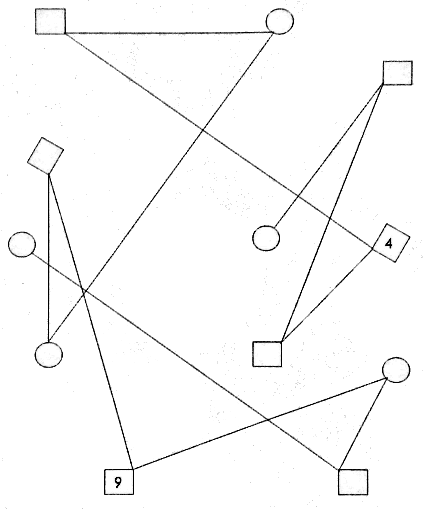
\includegraphics[width = 14 cm]{MC1}

\newpage

\noindent \textbf{Metacognitive Exercise 2}

\noindent Follow the lines as described with your not dominant hand.

\noindent 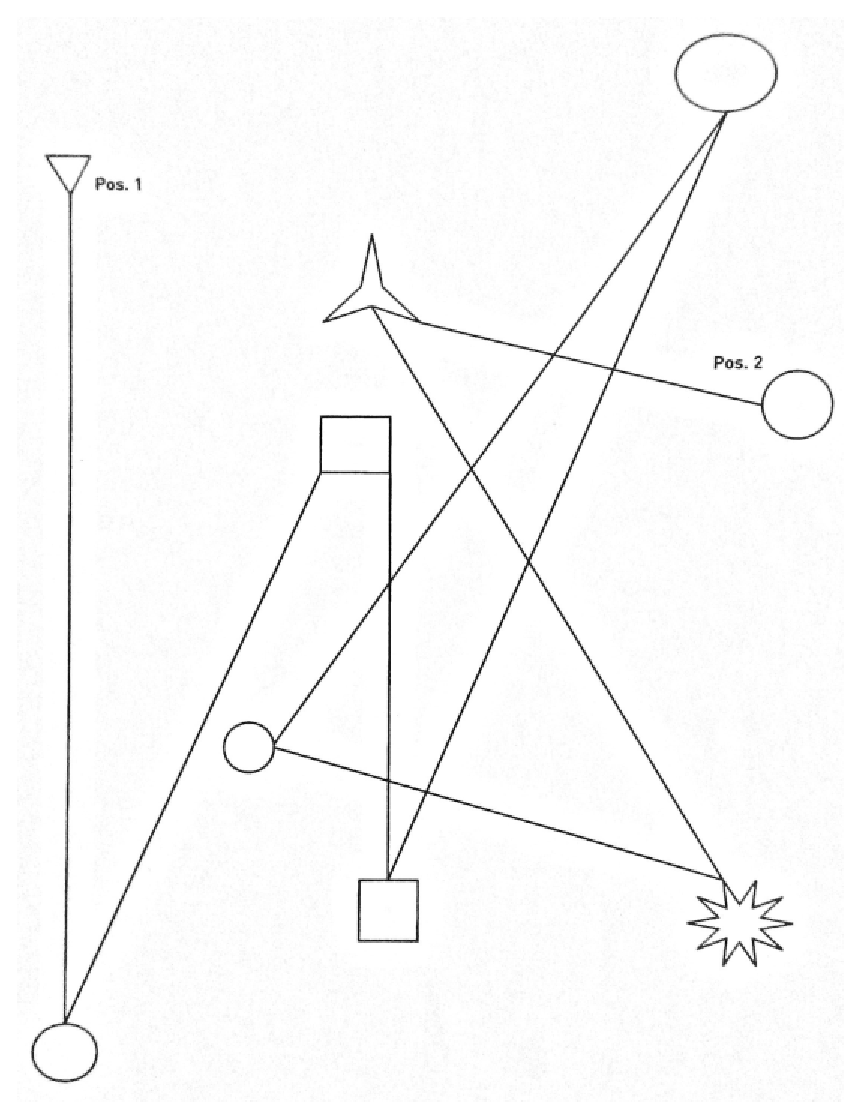
\includegraphics[width = 14 cm]{MC2}

\newpage


\noindent \textbf{Metacognitive Exercise 3}

\noindent Follow the letters in alphabetical order as described above. One letter appears twice, on purpose. Find your way by not always following the same path.

\noindent 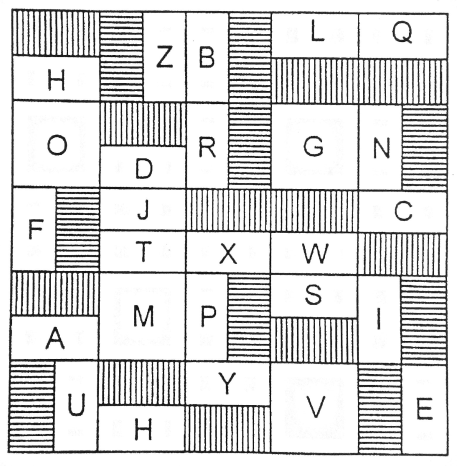
\includegraphics[width = 14 cm]{MC3}

\newpage

\section{Further Effects}

These exercises improve the capacity to {focus}\index{focus!training}. You will probably start to notice after some practice, how your awake state has been improved for the whole day.
Furthermore, they improve the endurance in the domain of thinking, but as well the {thinking speed will increase}.
After mid to long term practice, there may be improvement in {stress dominant traits} (ie. test anxiety, low self--esteem and impaired problem--thinking).

\section{A Possibility for Regulation of Stress}


One of the problems of people who are suffering from stress is that an unhindered self--sustained dynamic created a \emph{viscous circle}.\index{viscious circle}
This circle is very hard to break through.
In the case that there are already fatal symptoms or even syndromes, the measures for stress regulation or stimulus reduction, so to say lowering of negative stress are to be adapted carefully to the existing situation.

From this we see clearly, that certain schematics for solutions, the so called support measures %Christina fragen, Fachwort (stimulation measures?)
are often insufficient and irreal (because it's not fitting) for the given situation.

Then there are the inhibitions, the {obstructions} to be considered, coming from negative or sometimes even unreal thinking structures of the affected people. the countless  excuses are part of that dynamic, which tell you that seemingly a change can't be made. In all these cases, normally the \emph{inner will to change}\index{change!will to} is missing.

Metacognitive exercises are often a real way to break through a {viscous circle}. But it's then recommended to check the execution of the exercises and announce that fact beforehand. 


\end{document}